\documentclass[journal]{IEEEtran}

%----------------------------------------------------------------------------------------
% PACKAGES
%----------------------------------------------------------------------------------------
\usepackage{amsmath,amsfonts}
\usepackage{algorithmic}
\usepackage{algorithm}
\usepackage{array}
\usepackage[font=normalsize,labelfont=sf,textfont=sf]{subfig}
\usepackage{textcomp}
\usepackage{stfloats}
\usepackage{url}
\usepackage{verbatim}
\usepackage{graphicx}
\usepackage{cite}
\hyphenation{op-tical net-works semi-conduc-tor IEEE-Xplore}
\usepackage[
    colorlinks=true, 
    linkcolor=blue, 
    citecolor=blue,
    urlcolor=blue
]{hyperref}

%----------------------------------------------------------------------------------------
% DOCUMENT BODY
%----------------------------------------------------------------------------------------
\begin{document}

\title{Dynamic Scene Modeling and Rendering: A Survey of Methods and Applications}

\author{
  Yuwei~Zhao$^{1,2}$,
  Kaiyuan~Zhang$^{1,2}$,
  Yuxiang~Liu$^{1,2}$,
  Yilin~Zhang$^{1,2}$,
  and~Keqin~Zhang$^{1,2}$
\thanks{$^{1}$School of Computer Science and Technology, Ocean University of China, Qingdao 266100, China.}
\thanks{$^{2}$School of MPs \& EPs, Heriot-Watt University, Edinburgh EH14 4AS, UK.}
}

\maketitle

%----------------------------------------------------------------------------------------
\begin{figure*}[!t]
  \centering
  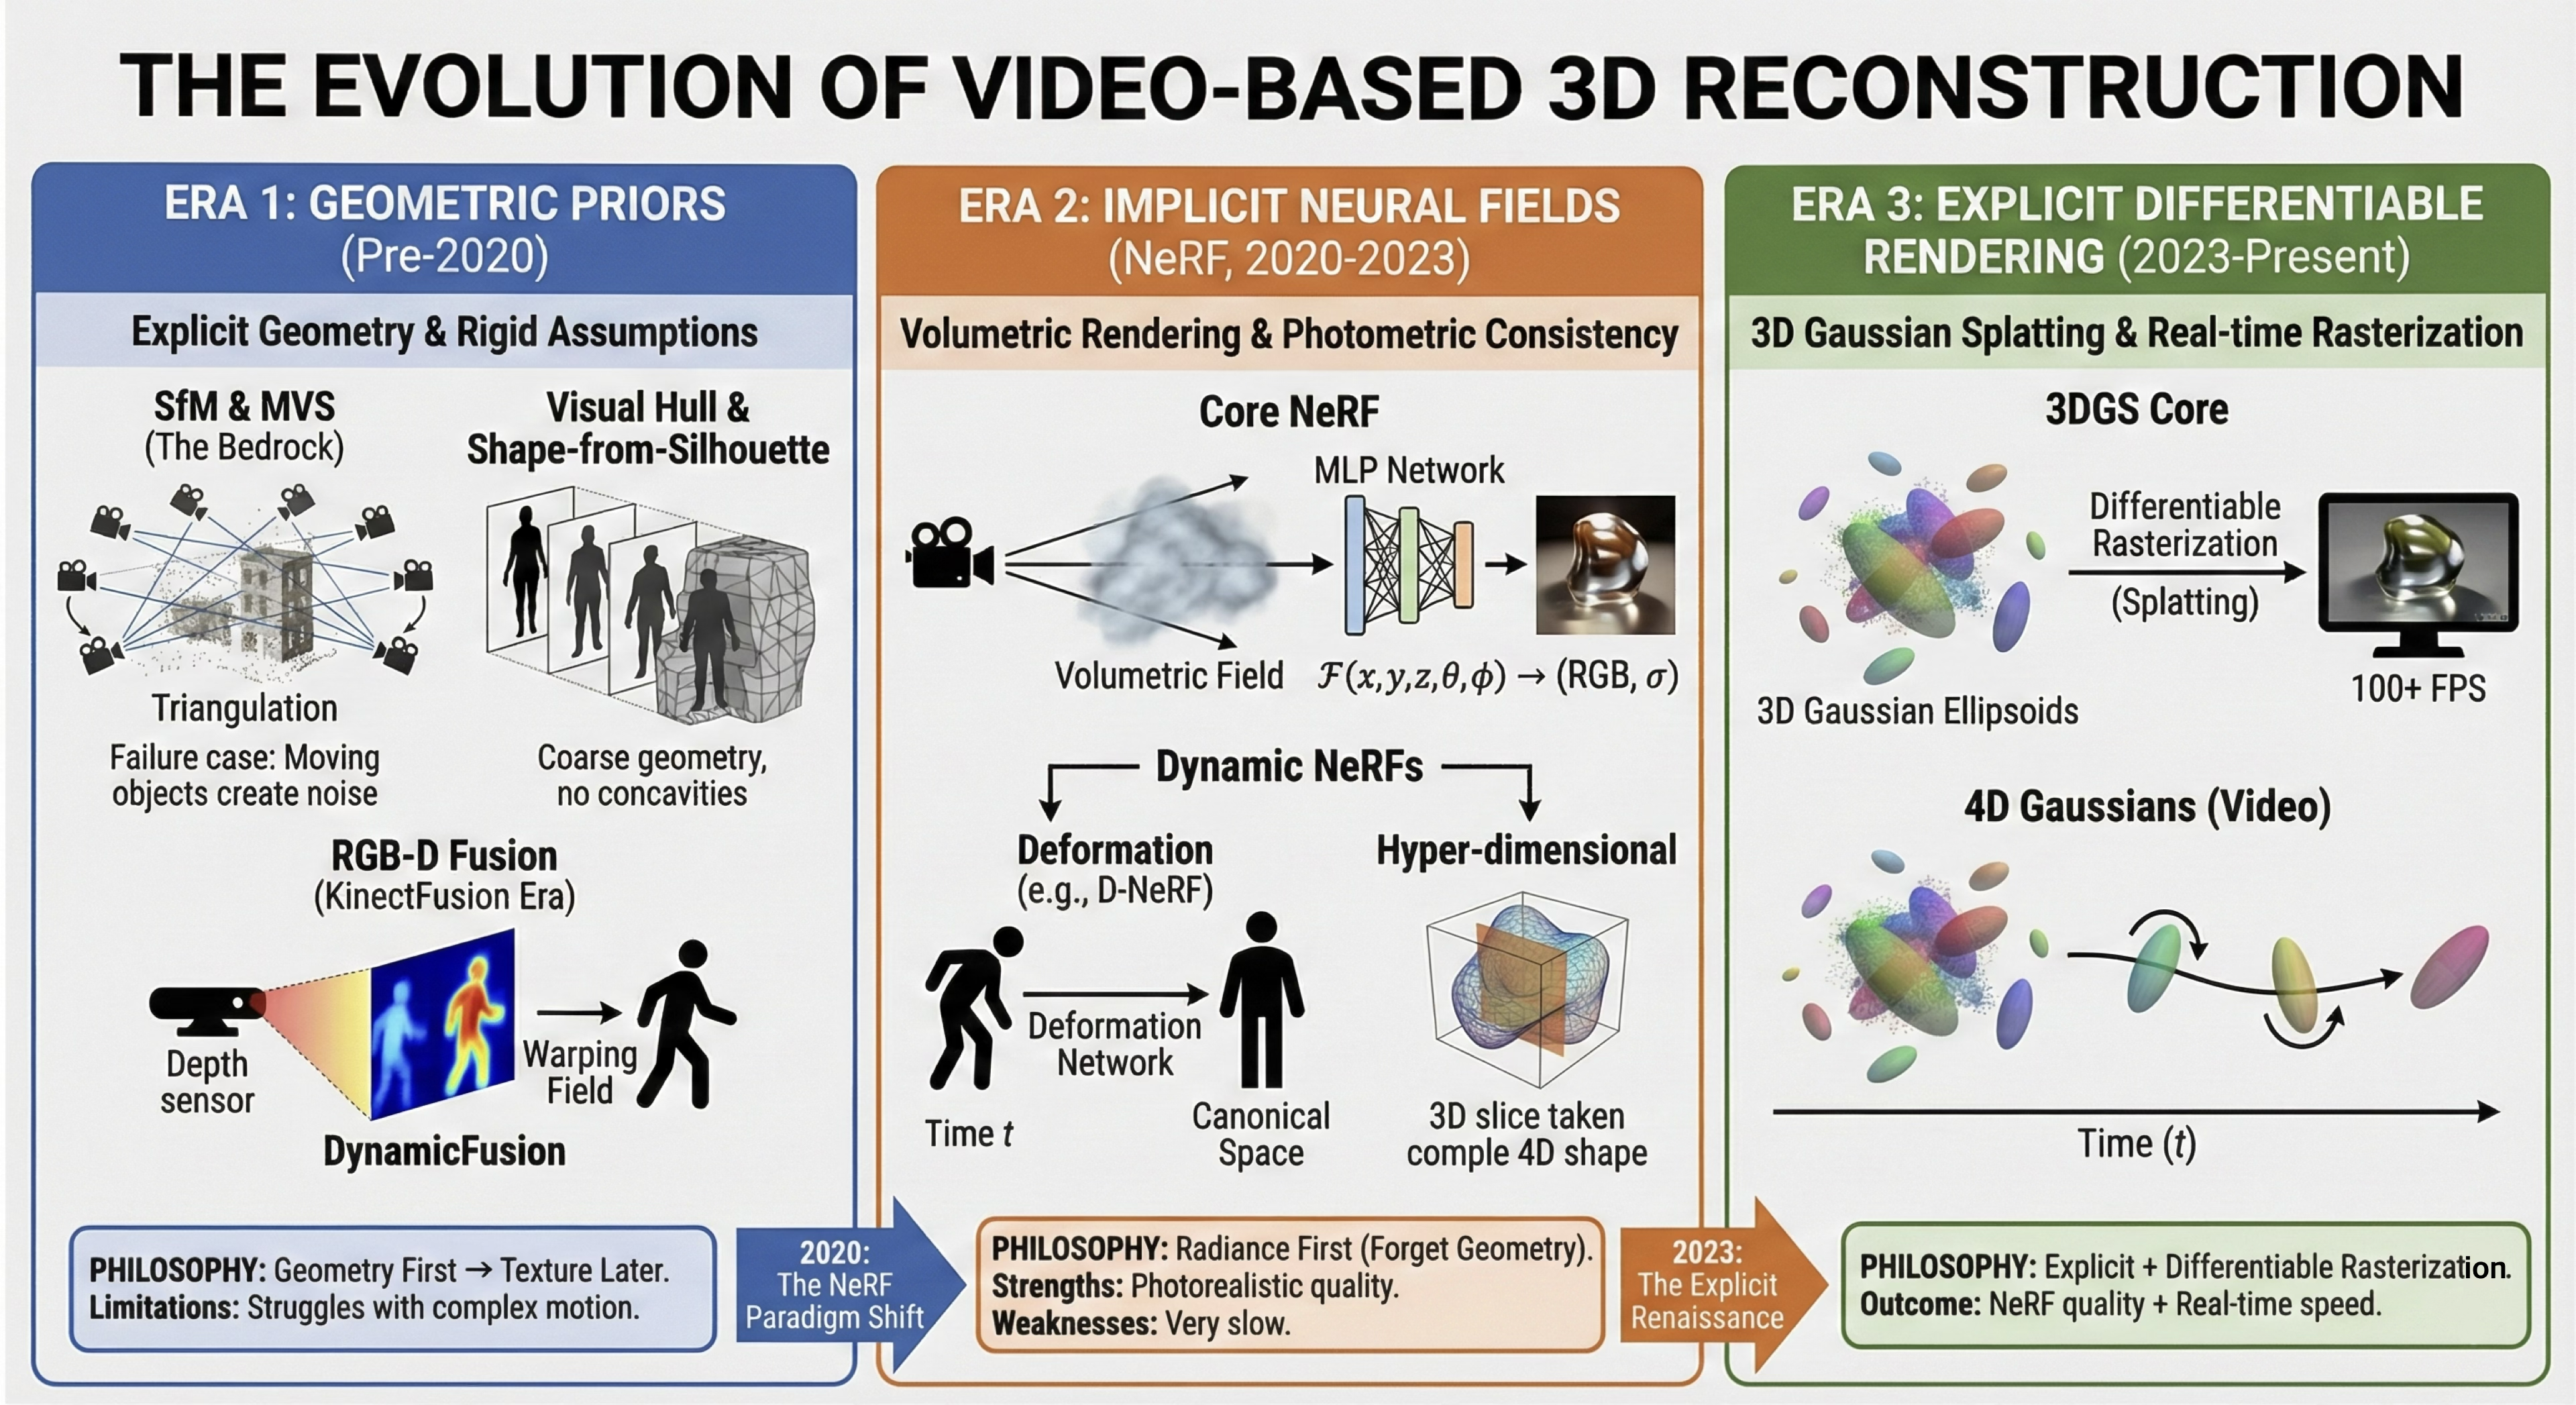
\includegraphics[width=0.95\textwidth]{./img/3d_reconstruction_evolution.png}
  \caption{Visualization of the evolution of video-based 3D reconstruction}
  \label{fig:evolution_3d_reconstruction}
\end{figure*}

%----------------------------------------------------------------------------------------
\begin{abstract}
    Dynamic scene modeling and reconstruction from video streams have witnessed a paradigm shift with the advent of Neural Radiance Fields (NeRF) and 3D Gaussian Splatting (3DGS). 
    While NeRF-based methods offer photorealistic quality via implicit neural representations, they often suffer from prohibitive training and rendering costs. 
    Recently, 3DGS has emerged as a powerful alternative, enabling real-time rendering through explicit splatting techniques, though it introduces new challenges regarding storage overhead and temporal consistency. 
    In this paper, we present a comprehensive survey of video-based 3D reconstruction methods, categorizing them into implicit and explicit approaches. 
    We systematically evaluate their trade-offs in terms of rendering quality, speed, and memory consumption across diverse scenarios. 
    Furthermore, we summarize the limitations of current state-of-the-art methods and discuss future directions. 
    Our compiled resources and code are available at \url{https://github.com/8arbatos/Academic-English-Group-Paper}.
\end{abstract}

%----------------------------------------------------------------------------------------
\begin{IEEEkeywords}
    3D Reconstruction, Dynamic Scene Modeling, Neural Radiance Fields (NeRF), Gaussian Splatting, Novel View Synthesis, Survey.
\end{IEEEkeywords}

%----------------------------------------------------------------------------------------
\section{Introduction}
\IEEEPARstart{W}{ith} the rapid advancement of virtual reality (VR), augmented reality (AR), and the Metaverse, the demand for photorealistic 3D content creation has surged exponentially. 
Dynamic scene modeling, which aims to reconstruct 3D geometry and appearance from 2D video streams, serves as a fundamental technology for these applications, enabling immersive telepresence, free-viewpoint video, and digital human avatars \cite{intro_metaverse}. 
Unlike static scene reconstruction, modeling dynamic scenes from video presents a highly ill-posed inverse problem due to the entanglement of object motion, topology changes, and time-variant lighting conditions.

Traditionally, 3D reconstruction relied on Structure-from-Motion (SfM) and Multi-View Stereo (MVS) algorithms \cite{colmap}. 
While these methods, such as COLMAP, provide robust camera pose estimation, they struggle to capture thin structures and view-dependent effects (e.g., reflections). 
More importantly, traditional pipelines typically assume a static world, making them brittle when applied to dynamic video sequences where geometry consistency is violated over time.

The field witnessed a paradigm shift with the introduction of \textbf{Neural Radiance Fields (NeRF)} \cite{nerf}. 
By representing scenes as implicit continuous functions parameterized by Multi-Layer Perceptrons (MLPs), NeRF achieved unprecedented rendering quality. 
Subsequent works, such as D-NeRF \cite{dnerf} and Nerfies \cite{nerfies}, extended this implicit paradigm to dynamic domains by introducing deformation fields to handle non-rigid motion. 
However, implicit methods suffer from prohibitive computational costs due to the extensive ray-marching sampling required during both training and inference, limiting their deployment in real-time applications.

Recently, \textbf{3D Gaussian Splatting (3DGS)} \cite{gaussian_splatting} has emerged as a compelling alternative, marking a return to explicit volumetric representations. 
By combining the differentiability of deep learning with the efficiency of rasterization-based rendering, 3DGS enables real-time rendering (100+ FPS) and fast training speeds. 
This breakthrough has triggered a new wave of research focused on extending Gaussian primitives to 4D spatiotemporal modeling \cite{4dgs, dynamic3dgs}, aiming to combine the efficiency of explicit representations with the flexibility of neural fields.

Despite the explosion of research papers in this domain, a systematic comparison between implicit (NeRF-based) and explicit (Gaussian-based) approaches for video modeling is lacking. 
In this survey, we provide a comprehensive review of the state-of-the-art methods for video-based 3D reconstruction. 
The main contributions of this paper are summarized as follows:

\begin{itemize}
    \item We propose a structured taxonomy of dynamic scene modeling methods, categorizing them into \textit{Deformation-based}, \textit{Spacetime-based}, and \textit{Hybrid} approaches across both implicit and explicit representations.
    \item We provide an in-depth analysis of the transition from NeRF to 3D Gaussian Splatting, highlighting the trade-offs between rendering quality, training efficiency, and storage overhead.
    \item We conduct a comparative evaluation of representative frameworks and discuss open challenges, including storage optimization and long-duration video modeling, to guide future research directions.
\end{itemize}

%----------------------------------------------------------------------------------------
\section{Preliminaries}
\subsection{Mathematical Formulation}
...

\subsection{Fundamentals of Neural Radiance Fields}
...

\subsection{Fundamentals of 3D Gaussian Splatting}
...

%----------------------------------------------------------------------------------------
\section{Taxonomy of Dynamic Scene Modeling}
\subsection{Implicit Deformation Fields (e.g., D-NeRF)}
...

\subsection{Spacetime Neural Fields (e.g., DyNeRF)}
...

\subsection{Dynamic Gaussian Splatting (e.g., 4D-GS)}
...

\subsection{Hybrid Representations}
...

%----------------------------------------------------------------------------------------
\section{Datasets and Metrics}
\subsection{Common Datasets (N3V, D-NeRF, etc.)}
...

\subsection{Evaluation Metrics (PSNR, SSIM, LPIPS, FPS)}
...

%----------------------------------------------------------------------------------------
\section{Comparative Analysis}
\subsection{Quantitative Benchmarks} % 放表格
...

\subsection{Qualitative Visual Comparisons} % 放对比图
...

\subsection{Efficiency Analysis (Time \& Memory)} % 讲速度和显存
...

%----------------------------------------------------------------------------------------
\section{Open Challenges and Future Directions}
\subsection{Storage Efficiency and Compression}
...

\subsection{Handling Long-Duration Videos}
...

\subsection{Integration with Generative Models}
...

%----------------------------------------------------------------------------------------
\section{Conclusion}
...

%----------------------------------------------------------------------------------------
% References
%----------------------------------------------------------------------------------------
\begin{thebibliography}{1}
  \bibliographystyle{IEEEtran}

  \bibitem{intro_metaverse}
  Apple Inc., {\it{Expression Estimation for Headsets Using Low-Profile Antenna and Impedance Characteristic Sensing}}.

  \bibitem{colmap}
  J. Schönberger, J.-M. Frahm, M. Pollefeys, P.-E. Sarlin, and S. Liu,
  {\it{COLMAP}}, [Online]. Available: https://colmap.github.io/index.html

  \bibitem{nerf}
  B. Mildenhall, P. P. Srinivasan, M. Tancik, J. T. Barron, R. Ramamoorthi, and R. Ng,
  ``NeRF: Representing Scenes as Neural Radiance Fields for View Synthesis,''
  {\it{arXiv preprint}}, arXiv:2003.08934, 2020.
  [Online]. Available: https://arxiv.org/abs/2003.08934

  \bibitem{dnerf}
  A. Pumarola, E. Corona, G. Pons-Moll, and F. Moreno-Noguer,
  ``D-NeRF: Neural Radiance Fields for Dynamic Scenes,''
  {\it{arXiv preprint}}, arXiv:2011.13961, 2020.
  [Online]. Available: https://arxiv.org/abs/2011.13961

  \bibitem{nerfies}
  K. Park, U. Sinha, J. T. Barron, S. Bouaziz, D. B. Goldman, S. M. Seitz, and R. Martin-Brualla,
  ``Nerfies: Deformable Neural Radiance Fields,''
  {\it{arXiv preprint}}, arXiv:2011.12948, 2021.
  [Online]. Available: https://arxiv.org/abs/2011.12948

  \bibitem{gaussian_splatting}
  J. Kerbl, A. Wang, F. Rousselle, and V. Koltun,
  ``3D Gaussian Splatting for Real-Time Radiance Field Rendering,''
  {\it{arXiv preprint}}, arXiv:2304.08914, 2023.
  [Online]. Available: https://arxiv.org/abs/2308.04079

  \bibitem{4dgs}
  G. Wu, T. Yi, J. Fang, L. Xie, X. Zhang, W. Wei, W. Liu, Q. Tian, and X. Wang,
  ``4D Gaussian Splatting for Real-Time Dynamic Scene Rendering,''
  {\it{arXiv preprint}}, arXiv:2310.08528, 2024.
  [Online]. Available: https://arxiv.org/abs/2310.08528

  \bibitem{dynamic3dgs}
  J. Luiten, G. Kopanas, B. Leibe, and D. Ramanan,
  ``Dynamic 3D Gaussians: Tracking by Persistent Dynamic View Synthesis,''
  {\it{arXiv preprint}}, arXiv:2308.09713, 2023.
  [Online]. Available: https://arxiv.org/abs/2308.09713
\end{thebibliography}

\newpage

%----------------------------------------------------------------------------------------
\section{Biography Section}
\begin{IEEEbiographynophoto}{Yuwei ZHAO}
Use $\backslash${\tt{begin\{IEEEbiographynophoto\}}} and the author name as the argument followed by the biography text.
\end{IEEEbiographynophoto}

%----------------------------------------------------------------------------------------
\end{document}